\documentclass{article}%
\usepackage[T1]{fontenc}%
\usepackage[utf8]{inputenc}%
\usepackage{lmodern}%
\usepackage{textcomp}%
\usepackage{lastpage}%
\usepackage{geometry}%
\geometry{left=2.5cm,top=1.5cm}%
\usepackage[dvipsnames]{xcolor}%
\usepackage{caption}%
\usepackage{float}%
\usepackage{array}%
\usepackage{colortbl}%
\usepackage{graphicx}%
\usepackage{slashbox}%
\usepackage{amsmath}%
\usepackage{xcolor}%
\usepackage{multirow}%
\usepackage{tcolorbox}%
\usepackage{ragged2e}%
%
%
%
\begin{document}%
\normalsize%
\section{Análisis Sísmico}%
\label{sec:AnlisisSsmico}%
\subsection{Factor de Zona}%
\label{subsec:FactordeZona}%
La ubicación de este proyecto es en la ciudad de Cusco, en el distrito de Cusco. Siguiendo los parámetros de la norma de diseño sismorresistente E.030 de octubre de 2018, la estructura se encuentra en la Zona 2%


\begin{table}[ht!]%
\begin{minipage}{0.55\textwidth}%
\caption{Factor de zona}%
\begin{tabular}{|>{\centering\arraybackslash}m{3.75cm}|>{\centering\arraybackslash}m{3.75cm}|}%
\hline%
\multicolumn{2}{|c|}{\textbf{FACTOR DE ZONA SEGÚN E{-}030}}\\%
\hline%
\textbf{ZONA}&\textbf{Z}\\%
\hline%
4&0.45\\%
\hline%
3&0.35\\%
\hline%
2\cellcolor[rgb]{ .949,  .949,  .949} &\textcolor[rgb]{ 1,  0,  0}{\textbf{0.25}}\cellcolor[rgb]{ .949,  .949,  .949} \\%
\hline%
1&0.10\\%
\hline%
\end{tabular}%
\end{minipage}%
\begin{minipage}{0.35\textwidth}%
\begin{center}%
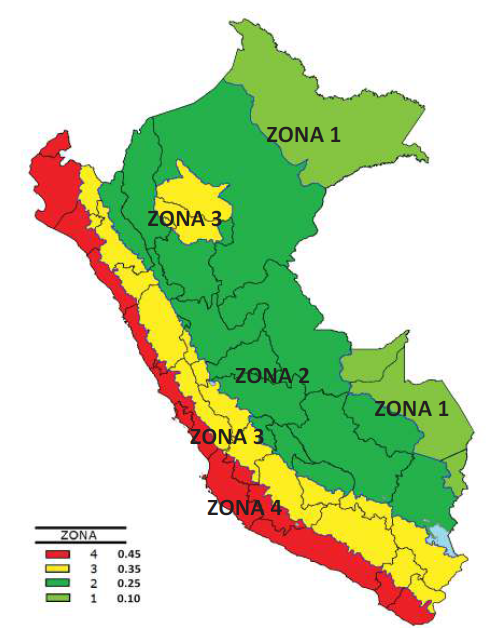
\includegraphics[width=4cm]{mapa_zona}%
\end{center}%
\end{minipage}%
\caption*{Fuente: E-030 (2018)}%
\end{table}

%
Este factor se interpreta como la aceleración máxima horizontal en el suelo rígido con una probabilidad de 10 \% de ser excedida en 50 años%
\subsection{Factor de suelo}%
\label{subsec:Factordesuelo}%
Este factor se interpreta como  un factor de modificación de la aceleración pico del suelo para un perfil determinado respecto al pefil tipo S1%


\begin{table}[ht!]%
\centering%
\caption{Factor de suelo}%
\begin{tabular}{|>{\centering\arraybackslash}m{3.75cm}|>{\centering\arraybackslash}m{2cm}|>{\centering\arraybackslash}m{2cm}|>{\centering\arraybackslash}m{2cm}|>{\centering\arraybackslash}m{2cm}|}%
\hline%
\multicolumn{5}{|c|}{\textbf{FACTOR DE SUELO SEGÚN E{-}030}}\\%
\hline%
\backslashbox{\textit{\textbf{ZONA}}}{\textit{\textbf{SUELO}}}&\textbf{S0}&\textbf{S1}&\textbf{S2}&\textbf{S3}\\%
\hline%
4&0.80&1.00\cellcolor[rgb]{ .949,  .949,  .949} &1.05&1.10\\%
\hline%
3&0.80&1.00\cellcolor[rgb]{ .949,  .949,  .949} &1.15&1.20\\%
\hline%
2\cellcolor[rgb]{ .949,  .949,  .949} &0.80\cellcolor[rgb]{ .949,  .949,  .949} &\textcolor[rgb]{ 1,  0,  0}{\textbf{1.00}}\cellcolor[rgb]{ .949,  .949,  .949} \cellcolor[rgb]{ .949,  .949,  .949} &1.20\cellcolor[rgb]{ .949,  .949,  .949} &1.40\cellcolor[rgb]{ .949,  .949,  .949} \\%
\hline%
1&0.80&1.00\cellcolor[rgb]{ .949,  .949,  .949} &1.60&2.00\\%
\hline%
\end{tabular}%
\caption*{Fuente: E-030 (2018)}%
\end{table}

%
\subsubsection{Periodos de suelo}%
\label{ssubsec:Periodosdesuelo}%
%


\begin{table}[ht!]%
\centering%
\caption{Periodos de suelo}%
\begin{tabular}{|>{\centering\arraybackslash} m{2cm}|>{\centering\arraybackslash}m{2cm}|>{\centering\arraybackslash}m{2cm}|>{\centering\arraybackslash}m{2cm}|>{\centering\arraybackslash}m{2cm}|}%
\cline{2-5}%
\multicolumn{1}{r|}{}&\multicolumn{4}{c|}{\textbf{PERIODO "Tp" y "Tl" SEGÚN E-030}}\\%
\cline{2-5}%
\multicolumn{1}{r|}{}&\multicolumn{4}{c|}{\textit{\textbf{Perfil de suelo}}}\\%
\cline{2-5}%
\multicolumn{1}{r|}{}&\textbf{S0}&\textbf{S1}&\textbf{S2}&\textbf{S3}\\%
\hline%
Tp&0.30&\textcolor[rgb]{ 1,  0,  0}{\textbf{0.40}}\cellcolor[rgb]{ .949,  .949,  .949} &0.60&1.00\\%
\hline%
Tl&3.00&\textcolor[rgb]{ 1,  0,  0}{\textbf{2.50}}\cellcolor[rgb]{ .949,  .949,  .949} &2.00&1.60\\%
\hline%
\end{tabular}%
\caption*{Fuente: E-030 (2018)}%
\end{table}

%
\subsection{Sistema Estructural}%
\label{subsec:SistemaEstructural}%
Después de realizar el análisis sísmico se determino que los sistemas estructurales en X, Y son:%
Muros y pórticos respectivamente.%


\begin{table}[ht!]%
\caption{coeficiente básico de reducción}%
\begin{tabular}{|>{\arraybackslash}m{10cm}| >{\centering\arraybackslash}m{4cm}|}%
\hline%
\multicolumn{2}{|c|}{\textbf{SISTEMAS ESTRUCTURALES}}\\%
\hline%
\textbf{Sistema Estructural}&\multicolumn{1}{m{4cm}|}{\textbf{Coeficiente Básico de Reducción Ro}}\\%
\hline%
\multicolumn{2}{|l|}{\textbf{Acero:}}\\%
\hline%
Porticos Especiales Resistentes a Momento (SMF)&8\\%
\hline%
Porticos Intermedios Resistentes a Momento (IMF)&5\\%
\hline%
Porticos Ordinarios Resistentes a Momento (OMF)&4\\%
\hline%
Porticos Ordinarios Resistentes a Momento (OMF)&7\\%
\hline%
Porticos Ordinarios Concentricamente Arrriostrados (OCBF)&4\\%
\hline%
Porticos Excentricamente Arriostrados (EBF)&8\\%
\hline%
\multicolumn{2}{|l|}{\textbf{Concreto Armado:}}\\%
\hline%
Porticos&8\\%
\hline%
Dual&7\\%
\hline%
De muros estructurales&6\\%
\hline%
Muros de ductilidad limitada&4\\%
\hline%
\textbf{Albañilería Armada o Confinada}&3\\%
\hline%
\textbf{Madera}&7\\%
\hline%
\end{tabular}%
\caption*{Fuente: E-30 (2018)}%
\end{table}

%
\subsection{Factor de Amplificación sísmica}%
\label{subsec:FactordeAmplificacinssmica}%
Las rigideces laterales pueden calcularse como la razon entre la fuerza cortante del entrepiso y el correspondiente desplazamiento relativo en el centro de masas, ambos evaluados para la misma condición de carga. \newline%
%
Se determina según el artículo 11 de la E{-}30%
\setlength{\jot}{0.5cm}%


\begin{figure}[h!]%
\caption{Factor de amplificación}%
\begin{minipage}{0.5\textwidth}%

    \begin{align*}
        &T< T_{P}         &   C&=2,5\cdot\left ( \frac{T_{P}}{T} \right )\\
        &T_{P}< T< T_{L}  &   C&=2,5\cdot\left ( \frac{T_{P}}{T} \right )\\
        &T> T_{L}         &   C&=2,5\cdot\left ( \frac{T_{P}\;T_{L}}{T^{2}} \right )
    \end{align*}%
\end{minipage}%
\begin{minipage}{0.4\textwidth}%
\centering%
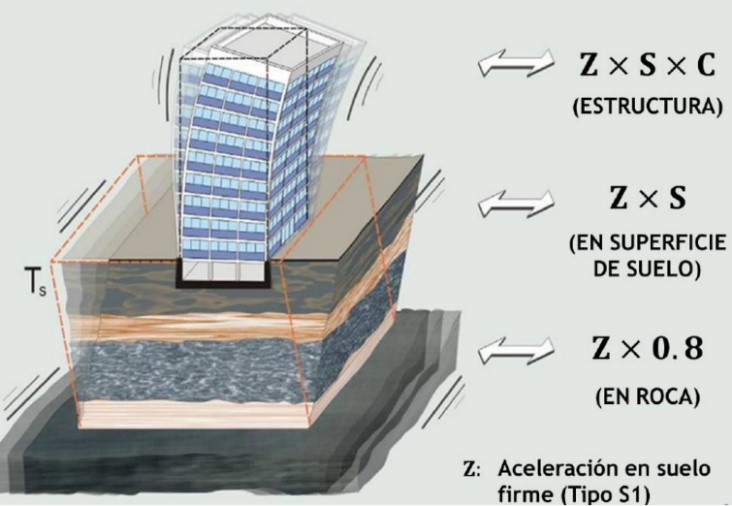
\includegraphics[width=6.5cm]{Amplificacion}%
\end{minipage}%
\caption*{Fuente: Muñoz (2020)}%
\end{figure}

%
\subsubsection{Factor de Importancia}%
\label{ssubsec:FactordeImportancia}%
%


\begin{table}[h!]%
\centering%
\caption{Factor de Uso o Importancia}%
\begin{tabular}{|>{\arraybackslash}m{3cm}|m{8cm}|>{\arraybackslash}m{2.8cm}|}%
\hline%
\multicolumn{3}{|c|}{\textbf{CATEGORIA DE LA EDIFICACION}}\\%
\hline%
\multicolumn{1}{|c|}{\textbf{CATEGORIA}}&\multicolumn{1}{|c|}{\textbf{DESCRIPCION}}&\multicolumn{1}{|c|}{\textbf{FACTOR U}}\\%
\hline%
\multirow{2}[4]{3cm}{A Edificaciones Escenciales}&A1: Establecimiento del sector salud (públicos y privados) del segundo y tercer nivel, según lo normado por el ministerio de salud.&\multicolumn{1}{>{\centering\arraybackslash}m{2.8cm}|}{Con aislamiento 1.0 y sin aislamiento 1.5.}\\%
\cline{2-3}%
&A2: Edificaciones escenciales para el manejo de las emergencias, el funcionamiento del gobierno y en general aquellas que puedan servir de refugio después de un desastre.\cellcolor[rgb]{1,  .949,  .8}&\multicolumn{1}{>{\centering\arraybackslash}m{2.8cm}|}{\textcolor[rgb]{ 1,  0,  0}{\textbf{1.50}}\cellcolor[rgb]{1,  .949,  .8}}\\%
\hline%
B Edificaciones Importantes &Edificaciones donde se reúnen gran cantidad de personas tales como cines, teatros, estadios, coliseos, centros comerciales, terminales de buses de pasajeros, establecimientos penitenciarios, o que guardan patrimonios valiosos como museos y bibliotecas.&\multicolumn{1}{>{\centering\arraybackslash}m{2.8cm}|}{1.30}\\%
\hline%
C Edificaciones Comunes&Edificaciones comunes tales como: viviendas, oficinas, hoteles, restaurantes, depósitos e instalaciones industriales cuya falla no acarree peligros adicionales de incendios o fugas de contaminantes.&\multicolumn{1}{>{\centering\arraybackslash}m{2.8cm}|}{1.00}\\%
\hline%
D Edificaciones temporales&Construcciones provisionales para depósitos, casetas y otras similares.&\multicolumn{1}{>{\centering\arraybackslash}m{2.8cm}|}{A criterio del proyectista}\\%
\hline%
\end{tabular}%
\caption*{Fuente: E-30 (2018)}%
\end{table}

%
\newpage%
\subsubsection{Irregularidad por Esquinas Entrantes}%
\label{ssubsec:IrregularidadporEsquinasEntrantes}%
\begin{tcolorbox}[colback=gray!5!white,colframe=cyan!75!black,fonttitle=\bfseries,title=Tabla N°9 E-030]%
\textit{La estructura se califica como irregular cuando los diafragmas tienen discontinuidades abruptas o variaciones importantes en rigidez, incluyendo aberturas mayores que 50\% del área bruta del diafragma.} \\ \textit{También  existe  irregularidad  cuando,  en  cualquiera de  los pisos y para cualquiera de las direcciones de análisis, se tiene alguna sección transversal del diafragma con un área neta resistente menor que 25\% del área de la sección transversal total de la misma dirección calculada con las dimensiones totales de la planta.}%
\end{tcolorbox}%


\begin{figure}[ht!]%
\centering%
\caption{Irregularidad por discontinuidad del diafragma}%
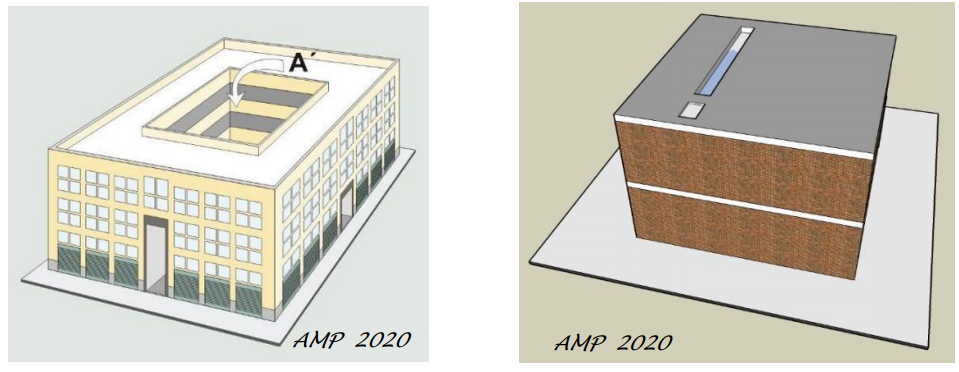
\includegraphics[scale=0.7]{i_diafragma.PNG}%
\caption*{\small Fuente: Muñoz (2020)}%
\end{figure}

%


\begin{table}[H]%
\centering%
\caption{Irregularidad por discontinuidad del diafragma (a)}%
\begin{tabular}{|ll|c|r}%
\cline{1-3}%
\multicolumn{2}{|l|}{Longitud del aligerado (L1)} & 7.51 & \multicolumn{1}{l}{m} \\%
\cline{1-3}%
\multicolumn{2}{|l|}{Espesor del aligerado (e1)} & 0.05 & \multicolumn{1}{l}{m} \\%
\cline{1-3}%
\multicolumn{2}{|l|}{Area del aligerado A1=L1$\cdot$ e1} & 0.38 & \multicolumn{1}{l}{$m^2$} \\%
\cline{1-3}%
\multicolumn{2}{|l|}{Longitud de la losa macisa (L2)} & 2.25 & \multicolumn{1}{l}{m} \\%
\cline{1-3}%
\multicolumn{2}{|l|}{Espesor de la losa macisa (e2)} & 0.2 & \multicolumn{1}{l}{m} \\%
\cline{1-3}%
\multicolumn{2}{|l|}{Area de la losa macisa A1=L1$\cdot$ e1} & 0.45 & \multicolumn{1}{l}{$m^2$} \\%
\cline{1-3}%
\multicolumn{2}{|l|}{Ratio} & 118.42 & \multicolumn{1}{l}{\%} \\%
\cline{1-3}%
\multicolumn{2}{|l|}{Ratio límite} & 25.00 & \multicolumn{1}{l}{\%} \\%
\cline{1-3}%
\multicolumn{2}{|l|}{Verificación} & \textcolor[rgb]{ .267,  .447,  .769}{\textbf{Regular}} & \multicolumn{1}{l}{} \\%
\cline{1-3}%
\end{tabular}%
\end{table}

%


\begin{table}[H]%
\centering%
\caption{Irregularidad por discontinuidad del diafragma (b)}%
\begin{tabular}{cccc}%
\hline%
\textbf{Abertura}&\textbf{Largo (m)}&\textbf{Ancho (m)}&\textbf{Área $m^2$}\\%
\hline%
1&4.02&2.30&9.25\\%
\hline%
2&1.10&2.30&2.53\\%
\hline%
3&1.20&19.00&22.80\\%
\hline%
&\multicolumn{2}{r}{Área total de aberturas:}&34.58 $m^2$\\%
&\multicolumn{2}{r}{Área total de la planta:}&120.41 $m^2$\\%
&\multicolumn{2}{r}{Ratio:}&28.72 \%\\%
&\multicolumn{2}{r}{Ratio límite:}&50.00 \%\\%
&\multicolumn{2}{r}{Verificación:}&\textcolor[rgb]{ .267,  .447,  .769} {Regular}\\%
\end{tabular}%
\end{table}

%
Las rigideces laterales pueden calcularse como la razon entre la fuerza cortante del entrepiso y el correspondiente desplazamiento relativo en el centro de masas, ambos evaluados para la misma condición de carga. \newline%
%
\end{document}